\documentclass[a4]{bioinfo}
\usepackage{url}
\usepackage{epsfig}
\usepackage{tabularx}

\bibliographystyle{bioinformatics}
\emergencystretch 2in

\copyrightyear{2014}
\pubyear{2014}
\title[JSAV: JavaScript Sequence Alignment Viewer]{Application Note:\\
JSAV: JavaScript Sequence Alignment Viewer}
\date{26th June, 2014}
\author[Martin]{Andrew C. R. Martin\mbox{${}^{\rm a}$}\footnote{to whom
    correspondence should be addressed}}
\address{\mbox{${}^{\rm a}$}Institute of Structural and Molecular Biology, 
Division of Biosciences,
University College London, Darwin Building, Gower Street, London WC1E 6BT}
\history{Received on XXXXX; revised on XXXXX; accepted on XXXXX}

\editor{Associate Editor: XXXXXXX}

\begin{document}
\maketitle

\begin{abstract}
\noindent{\bfseries Summary:} JSAV is designed as a simple-to-use
JavaScript component for displaying sequence alignments on web pages.
The display of sequences is highly configurable with options to allow
alternative colouring schemes, sorting of sequences, `dotifying'
repeated amino acids. An option is also available to submit selected
sequences to another web site or to other JavaScript code.  \\
\noindent{\bfseries Availability and Implementation:} 
JSAV is implemented purely in JavaScript making use of JQuery and
JQuery-UI. It does not use any HTML5 specific options to help with
browser compatibility. The code is documented using JSDOC
and is available from \url{http://www.bioinf.org.uk/software/jsav/} or
from GitHub \url{http://www.github.com/AndrewCRMartin/JSAV/}\\
\noindent{\bfseries Contact:} andrew@bioinf.org.uk --or--
andrew.martin@ucl.ac.uk
\end{abstract}


%%%%%%%%%%%%%%%%%%%%%%%%%%%%%%%%%%%%%%%%%%%%%%%%%%%%%%%%%%%%%%%%%%%%
\section{Introduction}
Viewing multiple sequence alignments (MSAs) is a fundamental
requirement in the analysis of protein sequences. MSAs allow us to
visualize conservation across protein families as well as unusual
features of particular sequences. As a result, there are a plethora of
tools for viewing sequence alignments. These range from tools which
provide attractive printed output, through standalone tools --- either
operating-system dependent, or independent --- to web-based viewers.

Two of the earlier such tools are HOMED\cite{stockwell:homed} and
MALIGNED\cite{clark:maligned} written for VAX/VMS workstations.
Neither seems to be actively maintained or easily available any
more. Other early viewers include GeneDoc\cite{nicholas:genedoc},
BioEdit and Seaview\cite{galtier:seaview}.

RnaViz\cite{derijk:rnaviz}, a program for visualizing RNA
secondary structure contains DCSE\cite{derijk:dcse}, an interactive
sequence alignment viewer and editor which can be used for protein
sequnece alignments, but is targeted at the examination of RNA. A
major problem in writing graphical software is the operating-system
dependency of many graphics libraries. CINEMA\cite{parrysmith:cinema}
was probably the first sequence alignment viewer and editor
implemented in Java, a platform independent programming language
allowing graphical interfaces to run on any operating system. More
recent software includes MPSA\cite{blanchet:mpsa} and ANTHEPROT\cite{deleage:antheprot}.
ClustalX\cite{thompson:clustalx} is a graphical user interface (GUI)
for the ClustalW multiple sequence aliugnment program providing an
integrated environment for aligning sequences and analyzing the
results. It is available for Linux, Mac and Windows platforms. Clustal
Omega is the most recent addition to the Clustal family, but at the
time of writing only has a command line interface --- a beta version
of a GUI is due to be released soon.

More recent developments include the Protein Family Alignment
Annotation Tool (PFAAT)\cite{johnson:pfaat} designed specifically for
family analysis and incorporating residue annotation tools as well as
integration with Jmol for protein structure display. Like CINEMA,
PFAAT is implemented in Java for operating system
independence. CLC~viewer is a recent free package written in Java for
Linux Mac and Windows. It contains a number of integrated tools and
acts as a core product for adding other features through a commercial
version of the software. A more
complete list is available on the web at
\url{http://en.wikipedia.org/wiki/List_of_alignment_visuzlization_software}.

Probably the most popular of the available tools is Jalview from Geoff
Barton's group in Dundee\cite{clamp:jalview}. Jalview is available in
two versions: a standalone Java application which is operating system
independent and provides many tools and facilities, and as a `light'
version (JalviewLight) --- a Java applet that can be embedded in a web
page. The latter responds to the need for web site developers to be
able to embed sequence alignment visualization tools into web pages.

However, in recent years there has been a gradual move away from using
Java applets in web pages. New HTML features such as the HTML5 Canvas
and powerful JavaScript libraries such as Bootstrap, JQuery and
JQuery-UI that provide an easier syntax for accessing elements of a
web page together with new widgets such as sliders and drag-and-drop
support, have overtaken Java as the method of choice for creating
interactive web sites with complex requirements. Such features are
used widely by commonly used popular web sites such as Google Mail,
Google Docs and Facebook.

To our knowledge, while there is an intention to port JalviewLight to
JavaScript, there are currently no JavaScript based sequence alignment
viewers available. To address this, we have developed JSAV (JavaScript
Sequence Alignment Viewer). JSAV is designed to be a lightweight
component that can easily be dropped into a web site to display and
manipulate a sequence alignment. It does not offer the ability to edit
the alignment, but does allow sorting and removing sequences as well
as integration with other web pages and local JavaScript code.



%%%%%%%%%%%%%%%%%%%%%%%%%%%%%%%%%%%%%%%%%%%%%%%%%%%%%%%%%%%%%%%%%%%%
\section{Implementation}

\begin{figure}
\footnotesize
\begin{verbatim}
var MySeqs = Array();

MySeqs.push({ id :"id1b1",  
   sequence :"SASSSVNYMYACREFGHIKLMNPTRSTVWY"});
MySeqs.push({ id :"id1a",   
   sequence :"SASSSTNYMYACDEFGHIKLMNPQRSTVWY"});
MySeqs.push({ id :"id2b1",  
   sequence :"SASSTCNYMTACDEEGHIKLMNP-RSTCWY"});

var MyOptions = Array();
MyOptions.sortable = true;
MyOptions.selectable = true;
MyOptions.deletable = true;
MyOptions.toggleDotify = true;
MyOptions.toggleNocolour = true;
MyOptions.consensus = true;
MyOptions.selectColour = true;

printJSAV('sequenceDisplay', MySeqs, MyOptions);
\end{verbatim}
\caption{\label{fig:code}Example code illustrating the creation of a
JavaScript array of sequence objects, the options and the call
necessary to create the alignment viewer.}
\end{figure}

\begin{figure}
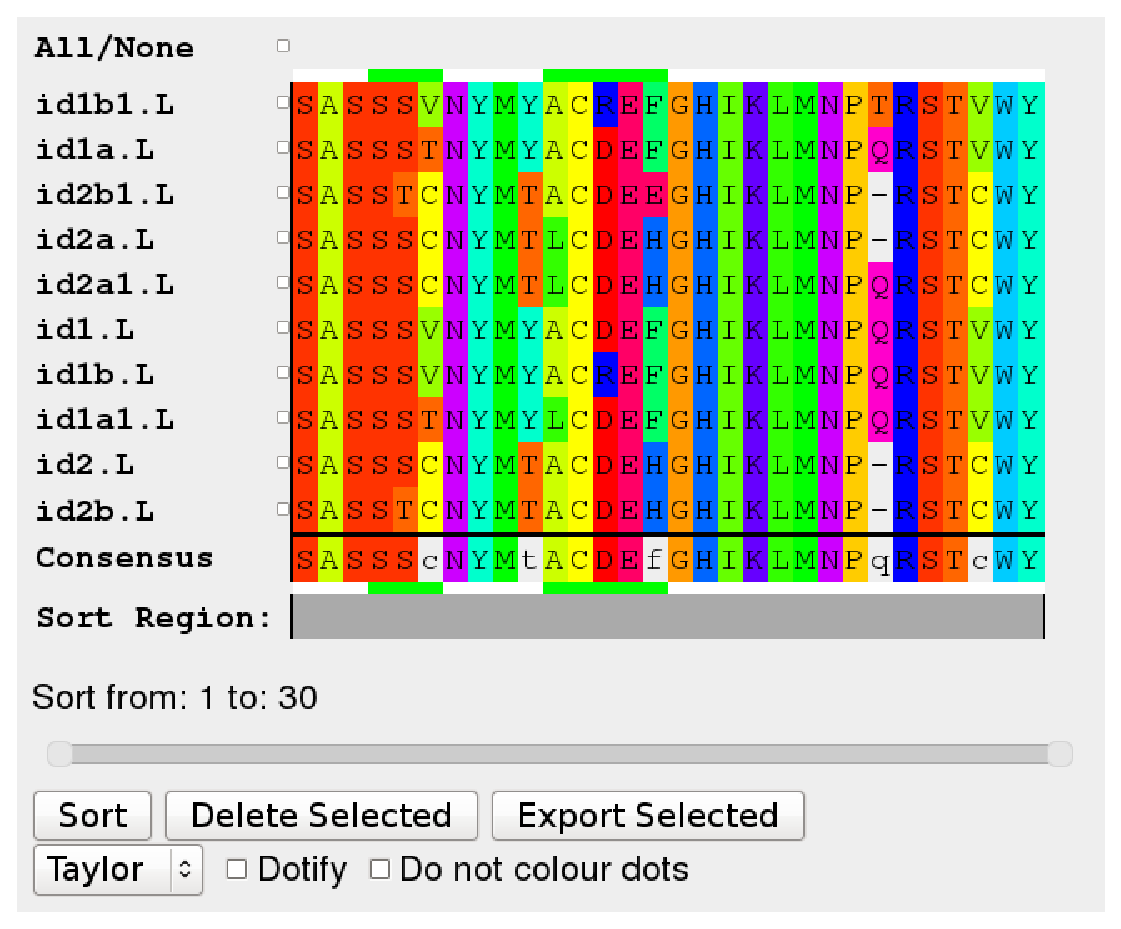
\epsfig{file=demo.eps,width=\columnwidth}
\caption{\label{fig:demo}Results of displaying sequences using 
  code of the form shown in Fig~\ref{fig:code}.}
\end{figure}

JSAV is implemented purely in JavaScript. JSAV employs the JQuery
library to ease access to elements of the HTML that it generates and
uses JQuery-UI to implement a two-value slider that is used to specify
a range of positions in the alignment.

As input, the code requires an array of JavaScript objects which
contain two elements: a unique identifier for a sequence and the
sequence itself --- all sequences must be pre-aligned.  Secondly a set
of options can be provided. These control the display and facilities
available to the end user of a web site.  A brief piece of example
code is shown in Fig~\ref{fig:code} with the results shown in
Fig~\ref{fig:demo}. 

The code allows the user to modify the view of the sequence in a
number of ways. The web-site provider has control over which of these
is available to the end user. First, the sequences can be sorted ---
the code selects the most representative sequence displaying that at
the top of the alignment followed by the most similar sequence and so
on. By default, sorting is performed across the whole sequence, but a
two-handled slider allows the range of positions to be sorted to
modified. Different colouring schemes are available duplicating those
provided in JalView. The alignment can also be `dotified', replacing
residues repeated between sequences with dots in order to emphasize
amino acid differences. Colouring of dotified residues can also be
switched off or on. Sequences can be selected and deleted from the
alignment; a consensus sequence can be displayed at the bottom of the
alignment and automatically updates when sequences are deleted. The
complete set of sequences, or a selected subset, can be submitted to
another web site, or passed to another JavaScript function for
integration with other tools. Tooltips are provided for each option
and all options are documented in detail on the web site.

%%%%%%%%%%%%%%%%%%%%%%%%%%%%%%%%%%%%%%%%%%%%%%%%%%%%%%%%%%%%%%%%%%%%
\section{Availability}
The software may be downloaded from
\url{http://www.bioinf.org.uk/software/jsav/} or from
\url{http://www.github.com/AndrewCRMartin/JSAV/} and used freely. The
web site provides demonstrations and full documentation. 

\bibliography{jsav}

\end{document}
